%%%%%%%%%%%%%%%%%%%%%%%%%%%%%%%%%%%%%
%                                   %
% Compile with XeLaTeX and biber    %
%                                   %
% Questions or comments:            %
%                                   %
% joshua dot mcneill at uga dot edu %
%                                   %
%%%%%%%%%%%%%%%%%%%%%%%%%%%%%%%%%%%%%

\documentclass{beamer}
  % Read in standard preamble (cosmetic stuff)
  %%%%%%%%%%%%%%%%%%%%%%%%%%%%%%%%%%%%%%%%%%%%%%%%%%%%%%%%%%%%%%%%
% This is a standard preamble used in for all slide documents. %
% It basically contains cosmetic settings.                     %
%                                                              %
% Joshua McNeill                                               %
% joshua dot mcneill at uga dot edu                            %
%%%%%%%%%%%%%%%%%%%%%%%%%%%%%%%%%%%%%%%%%%%%%%%%%%%%%%%%%%%%%%%%

% Beamer settings
% \usetheme{Berkeley}
\usetheme{CambridgeUS}
% \usecolortheme{dove}
% \usecolortheme{rose}
\usecolortheme{seagull}
\usefonttheme{professionalfonts}
\usefonttheme{serif}
\setbeamertemplate{bibliography item}{}

% Packages and settings
\usepackage{fontspec}
  \setmainfont{Charis SIL}
\usepackage{hyperref}
  \hypersetup{colorlinks=true,
              allcolors=blue}
\usepackage{graphicx}
  \graphicspath{{../../figures/}}
\usepackage[normalem]{ulem}
\usepackage{enumerate}

% Document information
\author{M. McNeill}
\title[FREN2001]{Français 2001}
\institute{\url{joshua.mcneill@uga.edu}}
\date{}

%% Custom commands
% Lexical items
\newcommand{\lexi}[1]{\textit{#1}}
% Gloss
\newcommand{\gloss}[1]{`#1'}
\newcommand{\tinygloss}[1]{{\tiny`#1'}}
% Orthographic representations
\newcommand{\orth}[1]{$\langle$#1$\rangle$}
% Utterances (pragmatics)
\newcommand{\uttr}[1]{`#1'}
% Sentences (pragmatics)
\newcommand{\sent}[1]{\textit{#1}}
% Base dir for definitions
\newcommand{\defs}{../definitions}


  % Packages and settings

  % Document information
  \subtitle[Révision: Examen 2]{Révision de l'examen 2}

\begin{document}
  % Read in the standard intro slides (title page and table of contents)
  \begin{frame}
    \titlepage
    \tiny{Office: % Basically a variable for office hours location
Gilbert 121\\
          Office hours: % Basically a variable for office hours
 lundi, mercredi, vendredi 10:10--11:10
}
  \end{frame}

  \begin{frame}{Choisis ta propre aventure \\ \gloss{Choose Your Own Adventure}}
    \hypertarget{début}{}
    \begin{columns}
      \column{0.5\textwidth}
        \begin{center}
          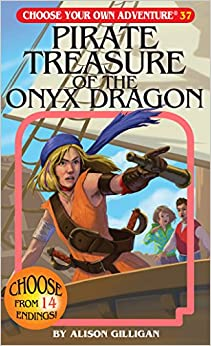
\includegraphics[scale=0.3]{aventure.jpg} \\
          La Caverne du temps
        \end{center}
      \column{0.5\textwidth}
        \begin{enumerate}
          \item \hyperlink{orale}{Compréhension orale} % remove this section
          \item \hyperlink{mort}{Passé composé}
          \item \hyperlink{sujets}{Sujets et métiers}
          \item \hyperlink{mort}{Subjonctif}
          \item \hyperlink{adjectifs}{Adjectifs}
          \item \hyperlink{mort}{Nourriture et boissons}
          \item \hyperlink{comparatifs}{Comparatifs et superlatifs}
        \end{enumerate}
    \end{columns}
  \end{frame}

% Prepositions de lieu (à droite de, en face de, près de, etc)
% Verbes (re, ir, pronominal, préférer, -oir)
% Adverbes (intensity, frequency, quantity)
  % Inject time into this

  \begin{frame}{Compréhension orale}
    \hypertarget{orale}{}
    Un gobelin commence à parler...
    \begin{columns}[t]
      \column{0.5\textwidth}
        \begin{enumerate}
          \item Benoît va...
          \begin{enumerate}
            \item faire du jogging...
            \item \alert<2->{faire du ski...}
            \item dîner...
          \end{enumerate}
          \item[] à \underline{\uncover<3->{2pm}}
          \item Claire va...
          \begin{enumerate}
            \item \alert<4->{aller au restaurant cher...}
            \item assister au match de football...
            \item nager...
          \end{enumerate}
          \item[] à \underline{\uncover<5->{6:30pm}}
        \end{enumerate}
      \column{0.5\textwidth}
        \begin{enumerate}
          \setcounter{enumi}{2}
          \item Ève va...
          \begin{enumerate}
            \item \alert<6->{se brosser les dents...}
            \item sortir à une fête avec ses amies...
            \item jouer au basket...
          \end{enumerate}
          \item[] à \underline{\uncover<7->{10am}}
        \end{enumerate}
        \begin{center}
          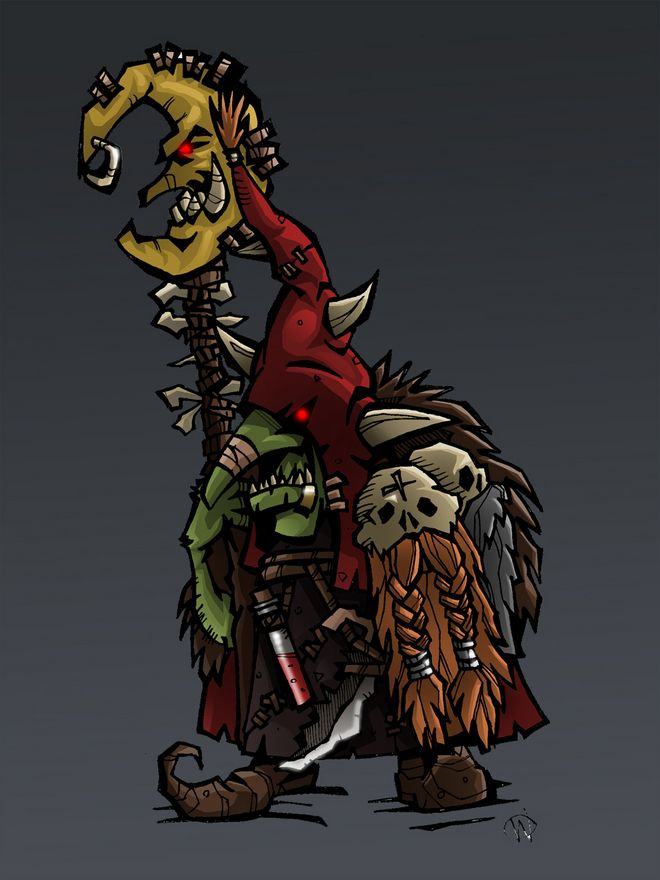
\includegraphics[scale=0.4]{gobelin.jpg}
        \end{center}
    \end{columns}
    Retourne au \hyperlink{début}{début}...
  \end{frame}

  \begin{frame}{Sujets et métiers}
    \hypertarget{sujets}{}
    Un mineur arrive.
    Il te demande quels sujets qu'il doit étudier pour ne plus être mineur...

    \vspace{0.25cm}
    \begin{columns}
      \column{0.6\textwidth}
        \small
        En tant que mineur, j'étudie les rochers, mais si je veux être écrivain, j'étudie \underline{\uncover<2->{les lettres, la littérature}}?
        D'accord, et je peux faire ça dans une \underline{\uncover<3->{bibliothèque}} ou un \underline{\uncover<3->{amphithéâtre}}?
        Parfait.
        Ma sœur est aussi mineure, mais elle étudie les mathématiques sur les ordinateurs pour être \underline{\uncover<4->{informaticienne}}.
        Est-ce une bonne idée?
        D'accord.
        Enfin, si je veux être assistant social, j'étudie \underline{\uncover<5->{l'anthropologie}}, \underline{\uncover<5->{la psychologie}}, \underline{\uncover<5->{la sociologie}}, ou \underline{\uncover<5->{le droit}}?
        Je ne sais pas si je veux travailler dans un \underline{\uncover<6->{bureau}}, mais j'aime aider les gens.

      \column{0.4\textwidth}
        \begin{center}
          
\includegraphics[scale=0.75]{mineur.jpg}
        \end{center}
    \end{columns}
    \vspace{0.25cm}
    En tout cas, tu peux revenir au \hyperlink{début}{début}...
  \end{frame}

  \begin{frame}{Adjectifs}
    \hypertarget{adjectifs}{}
    Il y a une grande orque âgée dans ce petit corridor gris.
    Elle ne sait pas bien ses adjectifs, alors tu dois les lui donner pour survivre...

    \vspace{0.25cm}
    \begin{columns}
      \column{0.6\textwidth}
        \small
        \underline{\uncover<2->{Cet}} (this) endroit est trop \underline{\uncover<3->{noir}} (black), mais je peux voir les gens.
        Par exemple, je regarde une sorcière, et \underline{\uncover<4->{cette}} (this) sorcière a un \underline{\uncover<5->{méchant}} (mean) mari.
        Et ce \underline{\uncover<6->{laid}} (ugly) gobelin, il pense qu'il est \underline{\uncover<7->{beau}} (handsome), mais moi je préfère regarder \underline{\uncover<8->{ces}} (these) baskets \underline{\uncover<9->{blanches}} (white), \underline{\uncover<10->{violettes}} (purple) et \underline{\uncover<11->{roses}} (pink).
        Je déteste les baskets.

      \column{0.4\textwidth}
        \begin{center}
          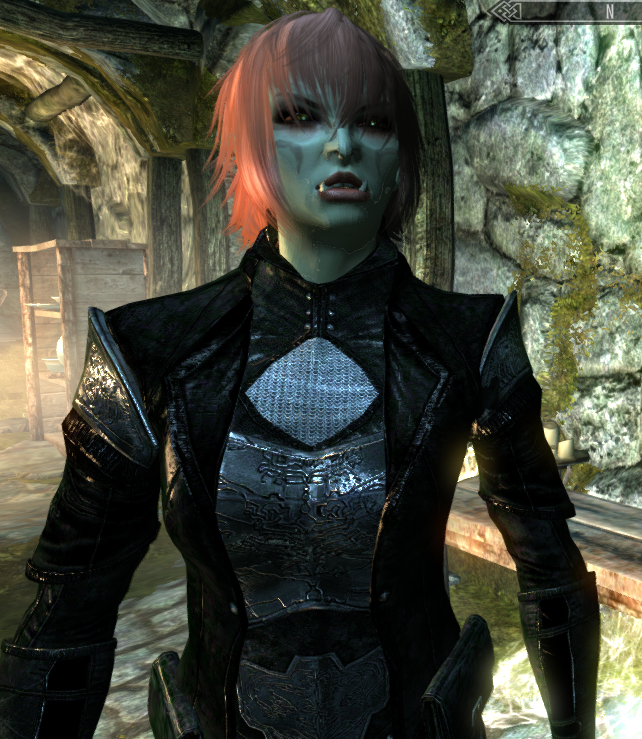
\includegraphics[scale=0.17]{orque.jpg}
        \end{center}
    \end{columns}
    \vspace{0.25cm}
    Mais tu es sympa.
    Tu peux revenir au \hyperlink{début}{début}...
  \end{frame}

  \begin{frame}{Comparatifs et superlatifs}
    \hypertarget{comparatifs}{}
    Un sorcier plus petit que Gandalf apparaît pour te faire faire des comparaisons...

    \vspace{0.25cm}
    \begin{columns}
      \column{0.6\textwidth}
        \scriptsize
        \begin{enumerate}
          \item David Attenborough est \underline{\uncover<2->{plus vieux que}} (older than) Mel Brooks par un mois.
          \item La cafétéria Snelling est \underline{\uncover<3->{meilleure que}} (better than) Bolton?
          \item La chimie est \underline{\uncover<4->{moins ennuyeuse que}} (less boring than) la comptabilité?
          \item Jordan Peele est \underline{\uncover<5->{le plus drôle}} (the funniest)?
          \item Les sandales sont \underline{\uncover<6->{moins chic que}} (less stylish than) les mocassins?
          \item Le rugby et le football américain sont \underline{\uncover<7->{les mêmes}} (the same).
        \end{enumerate}

      \column{0.4\textwidth}
        \begin{center}
          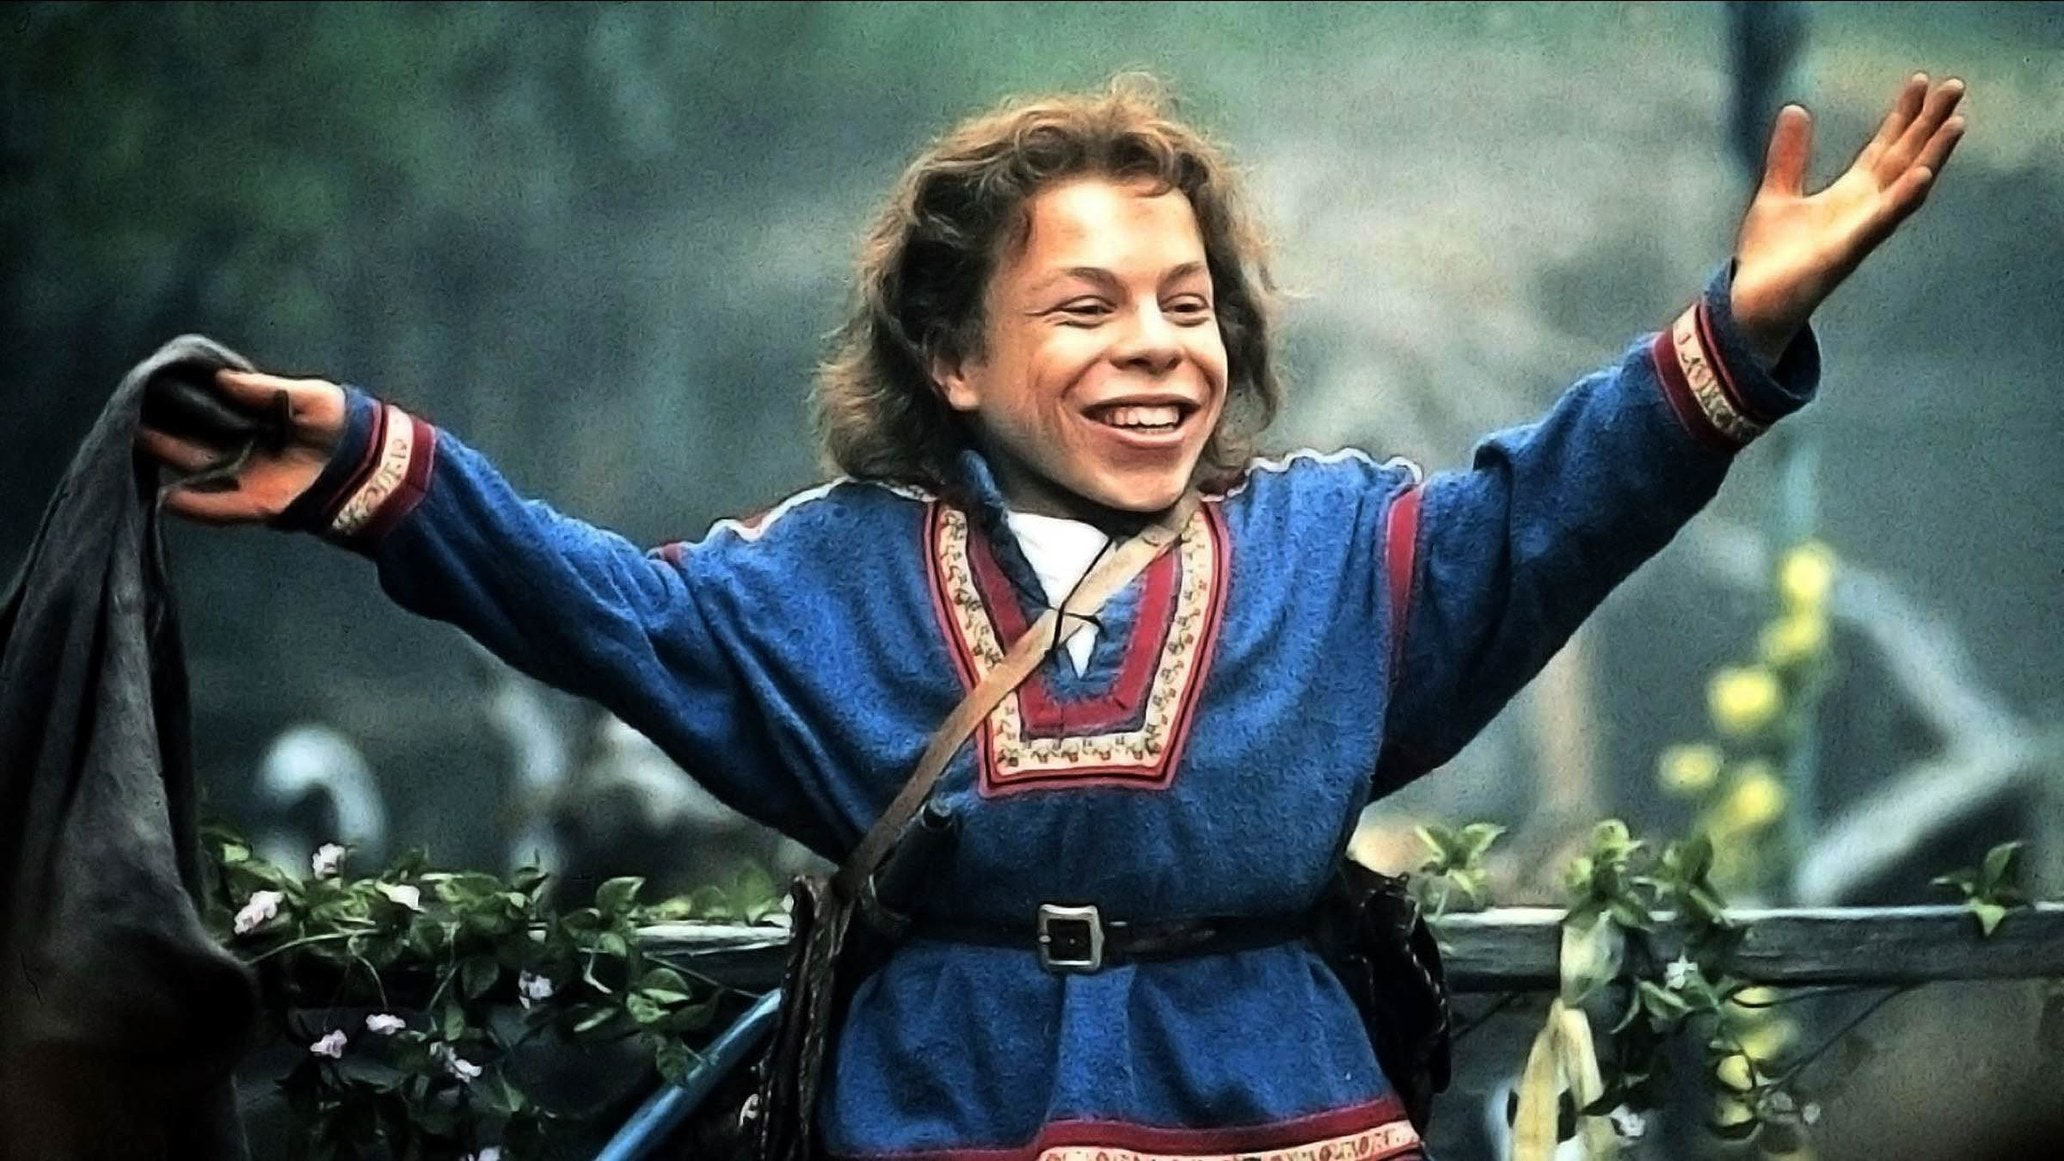
\includegraphics[scale=0.066]{willow.jpg}
        \end{center}
    \end{columns}
    \vspace{0.25cm}
    Tu peux revenir au \hyperlink{début}{début}...
  \end{frame}

  \begin{frame}{}
    \hypertarget{mort}{}
    Un fantôme maléfique \gloss{evil} apparaît!
    \begin{columns}
      \column{0.4\textwidth}
        \begin{center}
          
\includegraphics[scale=0.25]{phantom.jpg}
        \end{center}
      \column{0.6\textwidth}
        \begin{center}
          \Large{Tu meurs.} \\
          (c'est-à-dire que ça ne va pas être sur l'examen) \\
          \tinygloss{You die. (aka that won't be on the exam)}
        \end{center}

        \vspace{0.25cm}
        Retourne au \hyperlink{début}{début}...
    \end{columns}
  \end{frame}
\end{document}
